\documentclass[../main.tex]{subfiles}
\begin{document}
% \section{The angles}
\section{角}

% \subsection{Colour an angle: fill}
\subsection{\tkzcname{tkzFillAngle}命令:填充角}

% The simplest operation
% \begin{NewMacroBox}{tkzFillAngle}{\oarg{local options}\parg{A,O,B}}%
% $O$ is the vertex of the angle. $OA$ and $OB$ are the sides. Attention the angle
% is determined by the order of the points.
%
% \medskip
%
% \begin{tabular}{lll}%
% \toprule
% options             & default & definition                        \\
% \midrule
% \TOline{size}{1 cm}{this option determines the radius of the coloured angular
% sector.}
%
% \bottomrule
% \end{tabular}
%
% \medskip
% Of course, you have to add all the styles of \TIKZ, like the use of fill and
% shade\dots
% \end{NewMacroBox}
\begin{NewMacroBox}{tkzFillAngle}{\oarg{命令选项}\parg{A,O,B}}%
$O$是角顶点,$OA$和$OB$是两条边,点的顺序决定角的方向。

\medskip

\begin{tabular}{lll}%
\toprule
选项             & 默认值 & 含义                        \\
\midrule
\TOline{size}{1 cm}{着色扇形的半径}

\bottomrule
\end{tabular}

\medskip
可以使用所有有效的\TIKZ{}样式,如fill和shade等。
\end{NewMacroBox}

% \subsubsection{Example with \tkzname{size}}
\subsubsection{\tkzname{size}选项示例}
\begin{tkzexample}[latex=7cm,small]
\begin{tikzpicture}
  \tkzInit
  \tkzDefPoints{0/0/O,2.5/0/A,1.5/2/B}
  \tkzFillAngle[size=2cm, fill=gray!10](A,O,B)
  \tkzDrawLines(O,A O,B)
  \tkzDrawPoints(O,A,B)
\end{tikzpicture}
\end{tkzexample}

% \subsubsection{Changing the order of items}
\subsubsection{改变点的顺序示例}

\begin{tkzexample}[latex=7cm,small]
\begin{tikzpicture}
  \tkzInit
  \tkzDefPoints{0/0/O,2.5/0/A,1.5/2/B}
  \tkzFillAngle[size=2cm,fill=gray!10](B,O,A)
  \tkzDrawLines(O,A O,B)
  \tkzDrawPoints(O,A,B)
\end{tikzpicture}
\end{tkzexample}

\begin{tkzexample}[latex=7cm,small]
\begin{tikzpicture}[scale=0.75]
  \tkzInit
  \tkzDefPoints{0/0/O,5/0/A,3/4/B}
  % Don't forget {} to get, () to use
  \tkzFillAngle[size=4cm,left color=white,
                right color=red!50](A,O,B)
  \tkzDrawLines(O,A O,B)
  \tkzDrawPoints(O,A,B)
\end{tikzpicture}
\end{tkzexample}

\newpage
\subsection{\tkzcname{tkzFillAngles}命令:填充多个角}
% \begin{NewMacroBox}{tkzFillAngles}{\oarg{local options}\parg{A,O,B}\parg{A',O',B'}etc.}%
% With common options, there is a macro for multiple angles.
% \end{NewMacroBox}
\begin{NewMacroBox}{tkzFillAngles}{\oarg{命令选项}\parg{A,O,B}\parg{A',O',B'}等}%
绘制多个角。
\end{NewMacroBox}

% \subsubsection{Multiples angles}
\subsubsection{填充多个角示例}

\begin{tkzexample}[latex=7.5cm,small]
\begin{tikzpicture}[scale=0.7]
  \tkzDefPoint(0,0){B}
  \tkzDefPoint(8,0){C}
  \tkzDefPoint(0,8){A}
  \tkzDefPoint(8,8){D}
  \tkzDrawPolygon(B,C,D,A)
  \tkzDefTriangle[equilateral](B,C)
  \tkzGetPoint{M}
  \tkzInterLL(D,M)(A,B) \tkzGetPoint{N}
  \tkzDefPointBy[rotation=center N angle -60](D)
  \tkzGetPoint{L}
  \tkzInterLL(N,L)(M,B) \tkzGetPoint{P}
  \tkzInterLL(M,C)(D,L) \tkzGetPoint{Q}
  \tkzDrawSegments(D,N N,L L,D B,M M,C)
  \tkzDrawPoints(L,N,P,Q,M,A,D)
  \tkzLabelPoints[left](N,P,Q)
  \tkzLabelPoints[above](M,A,D)
  \tkzLabelPoints(L,B,C)
  \tkzMarkAngles(C,B,M B,M,C M,C,B
    D,L,N L,N,D N,D,L)
  \tkzFillAngles[fill=red!20,opacity=.2](C,B,M
    B,M,C M,C,B D,L,N L,N,D N,D,L)
\end{tikzpicture}
\end{tkzexample}

% \subsection{Mark an angle mark}
\subsection{标记角}

% More delicate operation because there are many options. The symbols used for
% marking in addition to those of \TIKZ\ are defined in the file
% |tkz-lib-marks.tex| and designated by the following
% characters:
在\TIKZ{}中,绘图选项非常丰富,本宏包又增加了需要的一些标记,它们定义在|tkz-lib-marks.tex|文件中,
主要的标记有:

\begin{tkzltxexample}[small]
|, ||,|||, z, s, x, o, oo
\end{tkzltxexample}

% Their definitions are as follows
它们的定义如下:

\begin{tkzltxexample}[vbox,small]
\pgfdeclareplotmark{||}
  %double bar
{%
  \pgfpathmoveto{\pgfqpoint{2\pgflinewidth}{\pgfplotmarksize}}
  \pgfpathlineto{\pgfqpoint{2\pgflinewidth}{-\pgfplotmarksize}}
  \pgfpathmoveto{\pgfqpoint{-2\pgflinewidth}{\pgfplotmarksize}}
  \pgfpathlineto{\pgfqpoint{-2\pgflinewidth}{-\pgfplotmarksize}}
  \pgfusepathqstroke
}
\end{tkzltxexample}

\newpage

\begin{tkzltxexample}[small]
  %triple bar
  \pgfdeclareplotmark{|||}
  {%
    \pgfpathmoveto{\pgfqpoint{0 pt}{\pgfplotmarksize}}
    \pgfpathlineto{\pgfqpoint{0 pt}{-\pgfplotmarksize}}
    \pgfpathmoveto{\pgfqpoint{-3\pgflinewidth}{\pgfplotmarksize}}
    \pgfpathlineto{\pgfqpoint{-3\pgflinewidth}{-\pgfplotmarksize}}
    \pgfpathmoveto{\pgfqpoint{3\pgflinewidth}{\pgfplotmarksize}}
    \pgfpathlineto{\pgfqpoint{3\pgflinewidth}{-\pgfplotmarksize}}
    \pgfusepathqstroke
  }
\end{tkzltxexample}

\vspace*{-10pt}

\begin{tkzltxexample}[small]
  % An bar slant
  \pgfdeclareplotmark{s|}
  {%
    \pgfpathmoveto{\pgfqpoint{-.70710678\pgfplotmarksize}%
                             {-.70710678\pgfplotmarksize}}
    \pgfpathlineto{\pgfqpoint{.70710678\pgfplotmarksize}%
                             {.70710678\pgfplotmarksize}}
    \pgfusepathqstroke
  }
\end{tkzltxexample}

\vspace*{-10pt}

\begin{tkzltxexample}[small]
  % An double bar slant
  \pgfdeclareplotmark{s||}
  {%
   \pgfpathmoveto{\pgfqpoint{-0.75\pgfplotmarksize}{-\pgfplotmarksize}}
   \pgfpathlineto{\pgfqpoint{0.25\pgfplotmarksize}{\pgfplotmarksize}}
   \pgfpathmoveto{\pgfqpoint{0\pgfplotmarksize}{-\pgfplotmarksize}}
   \pgfpathlineto{\pgfqpoint{1\pgfplotmarksize}{\pgfplotmarksize}}
   \pgfusepathqstroke
  }
\end{tkzltxexample}

\vspace*{-10pt}

\begin{tkzltxexample}[small]
  % z
  \pgfdeclareplotmark{z}
  {%
    \pgfpathmoveto{\pgfqpoint{0.75\pgfplotmarksize}{-\pgfplotmarksize}}
    \pgfpathlineto{\pgfqpoint{-0.75\pgfplotmarksize}{-\pgfplotmarksize}}
    \pgfpathlineto{\pgfqpoint{0.75\pgfplotmarksize}{\pgfplotmarksize}}
    \pgfpathlineto{\pgfqpoint{-0.75\pgfplotmarksize}{\pgfplotmarksize}}
    \pgfusepathqstroke
  }
\end{tkzltxexample}

\vspace*{-10pt}

\begin{tkzltxexample}[small]
  % s
  \pgfdeclareplotmark{s}
  {%
     \pgfpathmoveto{\pgfqpoint{0pt}{0pt}}
     \pgfpathcurveto
         {\pgfpoint{0pt}{0pt}}
         {\pgfpoint{-\pgfplotmarksize}{\pgfplotmarksize}}
         {\pgfpoint{\pgfplotmarksize}{\pgfplotmarksize}}
     \pgfpathmoveto{\pgfqpoint{0pt}{0pt}}
      \pgfpathcurveto
         {\pgfpoint{0pt}{0pt}}
         {\pgfpoint{\pgfplotmarksize}{-\pgfplotmarksize}}
         {\pgfpoint{-\pgfplotmarksize}{-\pgfplotmarksize}}
      \pgfusepathqstroke
  }
\end{tkzltxexample}

\vspace*{-10pt}

\begin{tkzltxexample}[small]
  % infinity
  \pgfdeclareplotmark{oo}
  {%
     \pgfpathmoveto{\pgfqpoint{0pt}{0pt}}
     \pgfpathcurveto
         {\pgfpoint{0pt}{0pt}}
         {\pgfpoint{.5\pgfplotmarksize}{1\pgfplotmarksize}}
         {\pgfpoint{\pgfplotmarksize}{0pt}}
     \pgfpathmoveto{\pgfqpoint{0pt}{0pt}}
      \pgfpathcurveto
         {\pgfpoint{0pt}{0pt}}
         {\pgfpoint{-.5\pgfplotmarksize}{1\pgfplotmarksize}}
         {\pgfpoint{-\pgfplotmarksize}{0pt}}
     \pgfpathmoveto{\pgfqpoint{0pt}{0pt}}
        \pgfpathcurveto
         {\pgfpoint{0pt}{0pt}}
         {\pgfpoint{.5\pgfplotmarksize}{-1\pgfplotmarksize}}
         {\pgfpoint{\pgfplotmarksize}{0pt}}
     \pgfpathmoveto{\pgfqpoint{0pt}{0pt}}
      \pgfpathcurveto
         {\pgfpoint{0pt}{0pt}}
         {\pgfpoint{-.5\pgfplotmarksize}{-1\pgfplotmarksize}}
         {\pgfpoint{-\pgfplotmarksize}{0pt}}
      \pgfusepathqstroke
  }
\end{tkzltxexample}

%                \tkzMarkAngle(B, A, C)
%
% Marque d'angle
% arc de cercle (simple/double/triple) et marque d'églité.
%
% Par défaut:
%                 arc       = simple
%                 mksize  = 1cm (rayon de l'arc)
%                 style traits pleins
%                 mkpos ?  position: 0.5 (position de la marque)
%                 mark rien du tout (ignoré si type est utilisé)
%
% Paramètres (optionnels)
%             arc     : l, ll, lll
%             mksize  : 1cm
%             gap     : 3pt
%             dist    : 1?
%             style   : type de traits
%             mkpos   : 0.5
%             mark    : none  , |, ||,|||, z, s, x, o, oo mais tous les
%  % symboles de tikz sont permis
\subsection{\tkzcname{tkzMarkAngle}命令:标记角}
% \begin{NewMacroBox}{tkzMarkAngle}{\oarg{local options}\parg{A,O,B}}%
% $O$ is the vertex. Attention the arguments vary according to the options.
% Several markings are possible. You can simply draw an arc or  add a mark on this
% arc. The style of the arc is chosen with the option \tkzname{arc}, the radius of
% the arc is given by \tkzname{mksize}, the arc can, of course, be colored.
%
% \medskip
%
% \begin{tabular}{lll}%
% \toprule
% options             & default & definition                        \\
% \midrule
% \TOline{arc}{l}{choice of l, ll and lll (single, double or triple).}
% \TOline{size}{1 cm}{arc radius.}
% \TOline{mark}{none}{choice of mark.}
% \TOline{mksize}{4pt}{symbol size (mark).}
% \TOline{mkcolor}{black}{symbol color (mark).}
% \TOline{mkpos}{0.5}{position of the symbol on the arc.}
% \end{tabular}
% \end{NewMacroBox}
\begin{NewMacroBox}{tkzMarkAngle}{\oarg{命令选项}\parg{A,O,B}}%
$O$是顶点,注意参数需随选项变化。
可以使用任意一种标记,甚至可以绘制一个圆弧,然后为该圆弧添加标记。
圆弧的样式通过\tkzname{arc}选项指定,圆弧的半径由\tkzname{mksize}选项指定。
当然,也可为圆弧着色。

\medskip

\begin{tabular}{lll}%
\toprule
选项             & 默认值 & 含义                        \\
\midrule
\TOline{arc}{l}{选择单线、双线或三线样式}
\TOline{size}{1 cm}{圆弧半径}
\TOline{mark}{无}{标记类型}
\TOline{mksize}{4pt}{标记符号尺寸}
\TOline{mkcolor}{black}{标记符号颜色}
\TOline{mkpos}{0.5}{标记位置}
\end{tabular}
\end{NewMacroBox}

% \subsubsection{Example with \tkzname{mark = x}}
\subsubsection{\tkzname{mark = x}选项示例}

\begin{tkzexample}[latex=6cm,small]
\begin{tikzpicture}[scale=.75]
  \tkzDefPoints{0/0/O,5/0/A,3/4/B}
  \tkzMarkAngle[size = 4cm,mark = x,
                 arc=ll,mkcolor = red](A,O,B)
  \tkzDrawLines(O,A O,B)
  \tkzDrawPoints(O,A,B)
\end{tikzpicture}
\end{tkzexample}

\newpage

\DeleteShortVerb{\|}

% \subsubsection{Example with \tkzname{mark =||}}
\subsubsection{\tkzname{mark =||}选项示例}

\MakeShortVerb{\|}
\begin{tkzexample}[latex=6cm,small]
\begin{tikzpicture}[scale=.75]
  \tkzDefPoints{0/0/O,5/0/A,3/4/B}
  \tkzMarkAngle[size = 4cm,mark = ||,
                arc=ll,mkcolor = red](A,O,B)
  \tkzDrawLines(O,A O,B)
  \tkzDrawPoints(O,A,B)
\end{tikzpicture}
\end{tkzexample}
\subsection{\tkzcname{tkzMarkAngles}命令:标记多个角}
% \begin{NewMacroBox}{tkzMarkAngles}{\oarg{local options}\parg{A,O,B}\parg{A',O',B'}etc.}%
% With common options, there is a macro for multiple angles.
% \end{NewMacroBox}
\begin{NewMacroBox}{tkzMarkAngles}{\oarg{命令选项}\parg{A,O,B}\parg{A',O',B'}等}%
对于具有相同选项的多个标记,可以一次标记多个角。
\end{NewMacroBox}

% \subsection{Label at an angle}
\subsection{\tkzcname{tkzLabelAngle}命令:标注角}

% \begin{NewMacroBox}{tkzLabelAngle}{\oarg{local options}\parg{A,O,B}}%
% There is only one option, dist (with or without unit), which can be replaced by
% the TikZ's pos option (without unit for the latter). By default, the value is in
% centimeters.
%
% \begin{tabular}{lll}%
% \toprule
% options             & default & definition                        \\
% \midrule
% \TOline{pos}{1}{ or dist, controls the distance from the top to the label.}
% \bottomrule
% \end{tabular}
%
% \medskip
% It is possible to move the label with all TikZ options : rotate, shift, below,
% etc.
% \end{NewMacroBox}
\begin{NewMacroBox}{tkzLabelAngle}{\oarg{命令选项}\parg{A,O,B}}%
该命令只有一个dist选项(带或不带单位),该选项可以被\TIKZ{}的选项(不带单位)替代,
默认情况下,其单位是cm。

\begin{tabular}{lll}%
\toprule
选项             & 默认值 & 含义                        \\
\midrule
\TOline{pos}{1}{或是dist,用于控制标注的距离}
\bottomrule
\end{tabular}

\medskip
可以使用\TIKZ{}的rotate、shift、below等选项调整标注的位置。
\end{NewMacroBox}

% \subsubsection{Example with \tkzname{pos}}
\subsubsection{\tkzname{pos}选项示例}

\begin{tkzexample}[latex=6cm,small]
\begin{tikzpicture}[scale=.75]
  \tkzDefPoints{0/0/O,5/0/A,3/4/B}
  \tkzMarkAngle[size = 4cm,mark = ||,
      arc=ll,color = red](A,O,B)%
  \tkzDrawLines(O,A O,B)
  \tkzDrawPoints(O,A,B)
  \tkzLabelAngle[pos=2,draw,circle,
      fill=blue!10](A,O,B){$\alpha$}
\end{tikzpicture}
\end{tkzexample}

\newpage

\begin{tkzexample}[latex=6.5cm,small]
\begin{tikzpicture}[rotate=30]
  \tkzDefPoint(2,1){S}
  \tkzDefPoint(7,3){T}
  \tkzDefPointBy[rotation=center S angle 60](T)
  \tkzGetPoint{P}
  \tkzDefLine[bisector,normed](T,S,P)
  \tkzGetPoint{s}
  \tkzDrawPoints(S,T,P)
  \tkzDrawPolygon[color=blue](S,T,P)
  \tkzDrawLine[dashed,color=blue,add=0 and 3](S,s)
  \tkzLabelPoint[above right](P){$P$}
  \tkzLabelPoints(S,T)
  \tkzMarkAngle[size = 1.8cm,mark = |,arc=ll,
                    color = blue](T,S,P)
  \tkzMarkAngle[size = 2.1cm,mark = |,arc=l,
                    color = blue](T,S,s)
  \tkzMarkAngle[size = 2.3cm,mark = |,arc=l,
                    color = blue](s,S,P)
  \tkzLabelAngle[pos = 1.5](T,S,P){$60^{\circ}$}%
  \tkzLabelAngles[pos = 2.7](T,S,s s,S,P){$30^{\circ}$}%
\end{tikzpicture}
\end{tkzexample}

\subsection{\tkzcname{tkzLabeAngles}命令:标注多个角}
% \begin{NewMacroBox}{tkzLabelAngles}{\oarg{local options}\parg{A,O,B}\parg{A',O',B'}etc.}%
% With common options, there is a macro for multiple angles.
% \end{NewMacroBox}
\begin{NewMacroBox}{tkzLabelAngles}{\oarg{命令选项}\parg{A,O,B}\parg{A',O',B'}等}%
当选项相同时,可以用该命令为多个角度添加标注。
\end{NewMacroBox}

% \subsection{Marking a right angle}
\subsection{\tkzcname{tkzMarkRightAngle}命令:标记直角}

% \begin{NewMacroBox}{tkzMarkRightAngle}{\oarg{local options}\parg{A,O,B}}%
% The \tkzname{german} option allows you to change the style of the drawing. The
% option \tkzname{size} allows to change the size of the drawing.
%
% \medskip
% \begin{tabular}{lll}%
% \toprule
% options             & default & definition         \\
% \midrule
% \TOline{german}{normal}{ german arc with inner point.}
% \TOline{size}{0.2}{ side size.}
% \end{tabular}
% \end{NewMacroBox}
\begin{NewMacroBox}{tkzMarkRightAngle}{\oarg{命令选项}\parg{A,O,B}}%
\tkzname{german}选项用于改变样式,
\tkzname{size}选项用于改变尺寸。

\medskip
\begin{tabular}{lll}%
\toprule
选项             & 默认值 & 含义         \\
\midrule
\TOline{german}{normal}{带内点的圆弧}
\TOline{size}{0.2}{ 标记边的尺寸}
\end{tabular}
\end{NewMacroBox}

% \subsubsection{Example of marking a right angle}
\subsubsection{直角标记示例}

\begin{tkzexample}[latex=6.5cm,small]
\begin{tikzpicture}
  \tkzDefPoints{0/0/A,3/1/B,0.9/-1.2/P}
  \tkzDefPointBy[projection = onto B--A](P)
  \tkzGetPoint{H}
  \tkzDrawLines[add=.5 and .5](P,H)
  \tkzMarkRightAngle[fill=blue!20,size=.5,draw](A,H,P)
  \tkzDrawLines[add=.5 and .5](A,B)
  \tkzMarkRightAngle[fill=red!20,size=.8](B,H,P)
  \tkzDrawPoints(A,B,P,H)
\end{tikzpicture}
\end{tkzexample}

\newpage

% \subsubsection{Example of marking a right angle, german style}
\subsubsection{使用german样式添加直角标记}

\begin{tkzexample}[latex=6cm,small]
\begin{tikzpicture}
  \tkzDefPoints{0/0/A,3/1/B,0.9/-1.2/P}
  \tkzDefPointBy[projection = onto B--A](P)
  \tkzGetPoint{H}
  \tkzDrawLines[add=.5 and .5](P,H)
  \tkzMarkRightAngle[german,size=.5,draw](A,H,P)
  \tkzDrawPoints[](A,B,P,H)
  \tkzDrawLines[add=.5 and .5,fill=blue!20](A,B)
  \tkzMarkRightAngle[german,size=.8](P,H,B)
\end{tikzpicture}
\end{tkzexample}

% \subsubsection{Mix of styles}
\subsubsection{混合样式}

\begin{tkzexample}[latex=6cm,small]
\begin{tikzpicture}[scale=0.75]
  \tkzDefPoint(0,0){A}
  \tkzDefPoint(4,1){B}
  \tkzDefPoint(2,5){C}
  \tkzDefPointBy[projection=onto B--A](C)
  \tkzGetPoint{H}
  \tkzDrawLine(A,B)
  \tkzDrawLine[add = .5 and .2,color=red](C,H)
  \tkzMarkRightAngle[,size=1,color=red](C,H,A)
  \tkzMarkRightAngle[german,size=.8,color=blue](B,H,C)
  \tkzFillAngle[opacity=.2,fill=blue!20,size=.8](B,H,C)
  \tkzLabelPoints(A,B,C,H)
  \tkzDrawPoints(A,B,C)
\end{tikzpicture}
\end{tkzexample}

% \subsubsection{Full example}
\subsubsection{完整示例}

\begin{tkzexample}[latex=6cm,small]
\begin{tikzpicture}[rotate=-90]
  \tkzDefPoint(0,1){A}
  \tkzDefPoint(2,4){C}
  \tkzDefPointWith[orthogonal normed,K=7](C,A)
  \tkzGetPoint{B}
  \tkzDrawSegment[green!60!black](A,C)
  \tkzDrawSegment[green!60!black](C,B)
  \tkzDrawSegment[green!60!black](B,A)
  \tkzDrawLine[altitude,dashed,color=magenta](B,C,A)
  \tkzGetPoint{P}
  \tkzLabelPoint[left](A){$A$}
  \tkzLabelPoint[right](B){$B$}
  \tkzLabelPoint[above](C){$C$}
  \tkzLabelPoint[left](P){$P$}
  \tkzLabelSegment[auto](B,A){$c$}
  \tkzLabelSegment[auto,swap](B,C){$a$}
  \tkzLabelSegment[auto,swap](C,A){$b$}
  \tkzMarkAngle[size=1cm,color=cyan,mark=|](C,B,A)
  \tkzMarkAngle[size=1cm,color=cyan,mark=|](A,C,P)
  \tkzMarkAngle[size=0.75cm,color=orange,mark=||](P,C,B)
  \tkzMarkAngle[size=0.75cm,color=orange,mark=||](B,A,C)
  \tkzMarkRightAngle[german](A,C,B)
  \tkzMarkRightAngle[german](B,P,C)
\end{tikzpicture}
\end{tkzexample}

\newpage

% \subsection{\tkzcname{tkzMarkRightAngles}}
\subsection{\tkzcname{tkzMarkRightAngles}命令:标记多个直角}

% \begin{NewMacroBox}{tkzMarkRightAngles}{\oarg{local options}\parg{A,O,B}\parg{A',O',B'}etc.}%
% With common options, there is a macro for multiple angles.
% \end{NewMacroBox}
\begin{NewMacroBox}{tkzMarkRightAngles}{\oarg{命令选项}\parg{A,O,B}\parg{A',O',B'}等}%
当选项相同时,使用该命令标记多个直角。
\end{NewMacroBox}

\vspace*{-10pt}

% \section{Angles tools}
\section{角度测量命令}

% \subsection{Recovering an angle \tkzcname{tkzGetAngle}}
\subsection{\tkzcname{tkzGetAngle}命令:计算角度}

% \begin{NewMacroBox}{tkzGetAngle}{\parg{name of macro}}%
% Assigns the value in degree of an angle to a macro. This macro retrieves
% \tkzcname{tkzAngleResult} and stores the result in a new macro.
%
% \medskip
%
% \begin{tabular}{lll}%
% \toprule
% arguments             & example & explication             \\
% \midrule
% \TAline{name of macro} {\tkzcname{tkzGetAngle}\{ang\}}{\tkzcname{ang} contains
% the value of the angle.}
% \end{tabular}
% \end{NewMacroBox}
\begin{NewMacroBox}{tkzGetAngle}{\parg{宏名称}}%
将角度值以度为单位存入指定宏,
可用\tkzcname{tkzAngleResult}命令得到角度值并存入指定宏。

\medskip

\begin{tabular}{lll}%
\toprule
参数             & 样例 & 含义             \\
\midrule
\TAline{宏名称} {\tkzcname{tkzGetAngle}\{ang\}}{\tkzcname{ang}保存了角度值(度)}
\end{tabular}
\end{NewMacroBox}

% \subsection{Example of the use of \tkzcname{tkzGetAngle}}
\subsubsection{\tkzcname{tkzGetAngle}命令示例}

% The point here is that $(AB)$ is the bisector of $\widehat{CAD}$, such that the
% $AD$ slope is zero. We recover the slope of $(AB)$ and then rotate twice.
直线$(AB)$是角$\widehat{CAD}$的角平分线,因此$AD$的斜率为0,
得到$(AB)$)的斜率后将其旋转2次。

\begin{tkzexample}[latex=6cm,small]
\begin{tikzpicture}
  \tkzInit
  \tkzDefPoint(1,5){A} \tkzDefPoint(5,2){B}
  \tkzDrawSegment(A,B)
  \tkzFindSlopeAngle(A,B) \tkzGetAngle{tkzang}
  \tkzDefPointBy[rotation= center A angle \tkzang](B)
  \tkzGetPoint{C}
  \tkzDefPointBy[rotation= center A angle - \tkzang](B)
  \tkzGetPoint{D}
  \tkzCompass[length=1,dashed,color=red](A,C)
  \tkzCompass[delta=10,brown](B,C)
  \tkzDrawPoints(A,B,C,D)
  \tkzLabelPoints(B,C,D)
  \tkzLabelPoints[above left](A)
  \tkzDrawSegments[style=dashed,color=orange!30](A,C A,D)
\end{tikzpicture}
\end{tkzexample}

% \subsection{Angle formed by three points}
\subsection{\tkzcname{tkzFindAngle}命令:计算三个点定义的角的角度}

% \begin{NewMacroBox}{tkzFindAngle}{\parg{pt1,pt2,pt3}}%
% The result is stored in a macro \tkzcname{tkzAngleResult}.
%
% \medskip
%
% \begin{tabular}{lll}%
% \toprule
% arguments     & example & explication     \\
% \midrule
% \TAline{(pt1,pt2,pt3)}
% {\tkzcname{tkzFindAngle}(A,B,C)}{\tkzcname{tkzAngleResult} gives the angle
% ($\overrightarrow{BA},\overrightarrow{BC}$)}
% \bottomrule
% \end{tabular}
%
% \medskip
% The result is between -180 degrees and +180 degrees. pt2 is the vertex and
% \tkzcname{tkzGetAngle} can retrieve the angle.
% \end{NewMacroBox}
\begin{NewMacroBox}{tkzFindAngle}{\parg{pt1,pt2,pt3}}%
结果保存在\tkzcname{tkzAngleResult}中。

\medskip

\begin{tabular}{lll}%
\toprule
参数     & 样例 & 说明     \\
\midrule
\TAline{(pt1,pt2,pt3)}
{\tkzcname{tkzFindAngle}(A,B,C)}{\tkzcname{tkzAngleResult}是
($\overrightarrow{BA},\overrightarrow{BC}$)之间的角度}
\bottomrule
\end{tabular}

\medskip
结果在-180度到+180度之间,pt2是顶点,
可以使用\tkzcname{tkzGetAngle}得到结果。
\end{NewMacroBox}

\newpage

% \subsubsection{Verification of angle measurement}
\subsubsection{角度测量示例}

\begin{tkzexample}[latex=7cm,small]
\begin{tikzpicture}[scale=.75]
  \tkzDefPoint(-1,1){A} \tkzDefPoint(5,2){B}
  \tkzDefEquilateral(A,B)
  \tkzGetPoint{C}
  \tkzDrawPolygon(A,B,C)
  \tkzFindAngle(B,A,C)
  \tkzGetAngle{angleBAC}
  \edef\angleBAC{\fpeval{round(\angleBAC)}}
  \tkzDrawPoints(A,B,C)
  \tkzLabelPoints(A,B)
  \tkzLabelPoint[right](C){$C$}
  \tkzLabelAngle(B,A,C){\angleBAC$^\circ$}
  \tkzMarkAngle[size=1.5cm](B,A,C)
\end{tikzpicture}
\end{tkzexample}

% \subsection{Example of the use of \tkzcname{tkzFindAngle}}
\subsection{角度计算示例}

\begin{tkzexample}[vbox,small]
\begin{tikzpicture}[scale=0.85]
  \tkzInit[xmin=-1,ymin=-1,xmax=7,ymax=7]
  \tkzClip
  \tkzDefPoint(0,0){O} \tkzDefPoint (6,0){A}
  \tkzDefPoint(5,5){B} \tkzDefPoint (3,4){M}
  \tkzFindAngle(A,O,M) \tkzGetAngle{an}
  \tkzDefPointBy[rotation=center O angle \an](A)
  \tkzGetPoint{C}
  \tkzDrawSector[fill = blue!50,opacity=.5](O,A)(C)
  \tkzFindAngle(M,B,A)   \tkzGetAngle{am}
  \tkzDefPointBy[rotation = center O angle \am](A)
  \tkzGetPoint{D}
  \tkzDrawSector[fill = red!50,opacity = .5](O,A)(D)
  \tkzDrawPoints(O,A,B,M,C,D)
  \tkzLabelPoints(O,A,B,M,C,D)
  \edef\an{\fpeval{round(\an,2)}}\edef\am{\fpeval{round(\am,2)}}
  \tkzDrawSegments(M,B B,A)
  \tkzText(4,2){$\widehat{AOC}=\widehat{AOM}=\an^{\circ}$}
  \tkzText(1,4){$\widehat{AOD}=\widehat{MBA}=\am^{\circ}$}
\end{tikzpicture}
\end{tkzexample}

\newpage

% \subsubsection{Determination of the three angles of a triangle}
\subsubsection{三角形内角计算示例}

\begin{tkzexample}[vbox,small]
\begin{tikzpicture}[scale=1.25,rotate=30]
  \tkzDefPoints{0.5/1.5/A, 3.5/4/B, 6/2.5/C}
  \tkzDrawPolygon(A,B,C)
  \tkzDrawPoints(A,B,C)
  \tkzLabelPoints[below](A,C)
  \tkzLabelPoints[above](B)
  \tkzMarkAngle[size=1cm](B,C,A)
  \tkzFindAngle(B,C,A) \tkzGetAngle{angleBCA}
  \edef\angleBCA{\fpeval{round(\angleBCA,2)}}
  \tkzLabelAngle[pos = 1](B,C,A){$\angleBCA^{\circ}$}
  \tkzMarkAngle[size=1cm](C,A,B)
  \tkzFindAngle(C,A,B) \tkzGetAngle{angleBAC}
  \edef\angleBAC{\fpeval{round(\angleBAC,2)}}
  \tkzLabelAngle[pos = 1.8](C,A,B){$\angleBAC^{\circ}$}
  \tkzMarkAngle[size=1cm](A,B,C)
  \tkzFindAngle(A,B,C) \tkzGetAngle{angleABC}
  \edef\angleABC{\fpeval{round(\angleABC,2)}}
  \tkzLabelAngle[pos = 1](A,B,C){$\angleABC^{\circ}$}
\end{tikzpicture}
\end{tkzexample}

% \subsection{Determining a slope}
\subsection{\tkzcname{tkzFindSlope}命令:计算斜率}

% It is a question of determining whether it exists, the slope of a straight line
% defined by two points. No verification of the existence is made.
斜率由直线上两个点确定,该命令不检测其存在性。

% \begin{NewMacroBox}{tkzFindSlope}{\parg{pt1,pt2}\marg{name of macro}}%
% The result is stored in a macro.
%
% \medskip
%
% \begin{tabular}{lll}%
% \toprule
% arguments             & example & explication                         \\
% \midrule
% \TAline{(pt1,pt2){pt3}} {\tkzcname{tkzFindSlope}(A,B)\{slope\}}{\tkzcname{slope}
% will give the result of $\frac{y_B-y_A}{x_B-x_A}$} \\
% \bottomrule
% \end{tabular}
%
% \medskip
% \tkzHandBomb{}Careful not to have $x_B=x_A$.
% \end{NewMacroBox}
\begin{NewMacroBox}{tkzFindSlope}{\parg{pt1,pt2}\marg{宏名称}}%
斜率保存在指定宏中。

\medskip

\begin{tabular}{lll}%
\toprule
参数             & 样例 & 说明                         \\
\midrule
\TAline{(pt1,pt2){pt3}} {\tkzcname{tkzFindSlope}(A,B)\{slope\}}{\tkzcname{slope}
通过$\frac{y_B-y_A}{x_B-x_A}$}计算 \\
\bottomrule
\end{tabular}

\medskip
\tkzHandBomb{}当$x_B=x_A$时,没有斜率。
\end{NewMacroBox}

\newpage

\begin{tkzexample}[latex=7cm,small]
\begin{tikzpicture}[scale=1.25]
  \tkzInit[xmax=4,ymax=5]\tkzGrid[sub]
  \tkzDefPoint(1,2){A} \tkzDefPoint(3,4){B}
  \tkzDefPoint(3,2){C} \tkzDefPoint(3,1){D}
  \tkzDrawSegments(A,B A,C A,D)
  \tkzDrawPoints[color=red](A,B,C,D)
  \tkzLabelPoints(A,B,C,D)
  \tkzFindSlope(A,B){SAB} \tkzFindSlope(A,C){SAC}
  \tkzFindSlope(A,D){SAD}
  \pgfkeys{/pgf/number format/.cd,fixed,precision=2}
  \tkzText[fill=Gold!50,draw=brown](1,4)%
    {The slope of (AB) is: $\pgfmathprintnumber{\SAB}$}
  \tkzText[fill=Gold!50,draw=brown](1,3.5)%
    {The slope of (AC) is: $\pgfmathprintnumber{\SAC}$}
  \tkzText[fill=Gold!50,draw=brown](1,3)%
    {The slope of (AD) is: $\pgfmathprintnumber{\SAD}$}
\end{tikzpicture}
\end{tkzexample}

% \subsection{Angle formed by a straight line with the horizontal axis \tkzcname{tkzFindSlopeAngle}}
\subsection{\tkzcname{tkzFindSlopeAngle}命令:计算直线与横轴夹角}

% Much more interesting than the last one. The result is between $-180$ degrees and
% $+180$ degrees.
结果在-180度与+180度之间。

% \begin{NewMacroBox}{tkzFindSlopeAngle}{\parg{A,B}}%
% Determines the slope of the straight line (AB). The result is stored in a macro
% \tkzcname{tkzAngleResult}.
%
% \medskip
% \begin{tabular}{lll}%
% \toprule
% arguments  & example & explication     \\
% \midrule
% \TAline{(pt1,pt2)} {\tkzcname{tkzFindSlopeAngle}(A,B)}{}
% \bottomrule
% \end{tabular}
%
% \medskip
% \tkzcname{tkzGetAngle} can retrieve the result. If retrieval is not necessary,
% you can use \tkzcname{tkzAngleResult}.
% \end{NewMacroBox}
\begin{NewMacroBox}{tkzFindSlopeAngle}{\parg{A,B}}%
计算直线$(AB)$的斜率并保存在\tkzcname{tkzAngleResult}命令中。

\medskip
\begin{tabular}{lll}%
\toprule
参数  & 样例 & 说明     \\
\midrule
\TAline{(pt1,pt2)} {\tkzcname{tkzFindSlopeAngle}(A,B)}{}
\bottomrule
\end{tabular}

\medskip
用\tkzcname{tkzGetAngle}保存结果并命名
\end{NewMacroBox}

% \subsubsection{Folding}
\subsubsection{折叠示例}

\begin{tkzexample}[latex=7cm,small]
\begin{tikzpicture}
  \tkzDefPoint(1,5){A}
  \tkzDefPoint(5,2){B}
  \tkzDrawSegment(A,B)
  \tkzFindSlopeAngle(A,B)
  \tkzGetAngle{tkzang}
  \tkzDefPointBy[rotation=center A angle \tkzang](B)
  \tkzGetPoint{C}
  \tkzDefPointBy[rotation=center A angle - \tkzang](B)
  \tkzGetPoint{D}
  \tkzCompass[orange,length=1](A,C)
  \tkzCompass[orange,delta=10](B,C)
  \tkzDrawPoints(A,B,C,D)
  \tkzLabelPoints(B,C,D)
  \tkzLabelPoints[above left](A)
  \tkzDrawSegments[style=dashed,color=orange](A,C A,D)
\end{tikzpicture}
\end{tkzexample}

\newpage

% \subsubsection{Example of the use of \tkzcname{tkzFindSlopeAngle}}
\subsubsection{中点计算示例}

% Here is another version of the construction of a mediator
% 这是计算中点的另一个实例。

\begin{tkzexample}[latex=7cm,small]
\begin{tikzpicture}
  \tkzInit
  \tkzDefPoint(0,0){A}
  \tkzDefPoint(3,2){B}
  \tkzDefLine[mediator](A,B)
  \tkzGetPoints{I}{J}
  \tkzCalcLength[cm](A,B)
  \tkzGetLength{dAB}
  \tkzFindSlopeAngle(A,B)
  \tkzGetAngle{tkzangle}
  \begin{scope}[rotate=\tkzangle]
    \tikzset{arc/.style={color=gray,delta=10}}
    \tkzDrawArc[orange,R,arc](B,3/4*\dAB)(120,240)
    \tkzDrawArc[orange,R,arc](A,3/4*\dAB)(-45,60)
    \tkzDrawLine(I,J)
    \tkzDrawSegment(A,B)
  \end{scope}
  \tkzDrawPoints(A,B,I,J)
  \tkzLabelPoints(A,B) \tkzLabelPoints[right](I,J)
\end{tikzpicture}
\end{tkzexample}

\end{document}
\endinput
